\documentclass[12pt]{article}

\usepackage{amsmath}
\usepackage{amsthm}
\usepackage{amssymb}
\usepackage{fancyhdr}
\usepackage{tikz}
\usepackage{float}
\pagestyle{plain}
\theoremstyle{definition}
\usetikzlibrary{calc}

\tikzset{node distance=3cm, auto}

\author{Evgeny Kotelnikov}
\title{Exercises for Chapter 4}
\date{}

\begin{document}
\maketitle

\begin{enumerate}
  \item[6.]
    \begin{enumerate}
      \item \hfill 
            \begin{figure}[H]
              \centering
              \begin{tikzpicture}
                \node (1)              {$1$};
                \node (2) [right of=1] {$2$};
                \node (3) [right of=2] {$3$};
                \draw[->] (1) to node {} (2);
                \draw[->] (2) to node {} (3);
              \end{tikzpicture}
            \end{figure}
            No equations.

      \item \hfill
            \begin{figure}[H]
              \centering
              \begin{tikzpicture}
                \node (1)              {$1$};
                \node (2) [right of=1] {$2$};
                \node (3) [right of=2] {$3$};
                \draw[->,transform canvas={yshift=0.6ex}]  (1) to node {$f$} (2);
                \draw[->,transform canvas={yshift=-0.6ex}] (1) to node[anchor=north] {$g$} (2);
                \draw[->] (2) to node {} (3);
              \end{tikzpicture}
            \end{figure}
            Equations: $f = g$.

      \item \hfill
            \begin{figure}[H]
              \centering
              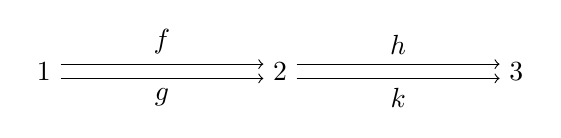
\begin{tikzpicture}
                \node (1)              {$1$};
                \node (2) [right of=1] {$2$};
                \node (3) [right of=2] {$3$};
                \draw[->,transform canvas={yshift=0.6ex}]  (1) to node {$f$} (2);
                \draw[->,transform canvas={yshift=-0.6ex}] (1) to node[anchor=north] {$g$} (2);
                \draw[->,transform canvas={yshift=0.6ex}] (2) to node {$h$} (3);
                \draw[->,transform canvas={yshift=-0.6ex}] (2) to node[anchor=north] {$k$} (3);
              \end{tikzpicture}
            \end{figure}
            Equations: $f = g$, $h = k$.

      \item \hfill
            \begin{figure}[H]
              \centering
              \begin{tikzpicture}
                \node (1)              {$1$};
                \node (2) [right of=1] {$2$};
                \node (3) [below of=2] {$3$};
                \draw[->] (1) to node {$f$} (2);
                \draw[<-] (3) to node {$g$} (1);
                \draw[<-] (2) to node {$h$} (3);
              \end{tikzpicture}
            \end{figure}
            Equations: $f = h \circ g$.
       \end{enumerate}
    $\mathbf{3}$ is free.

  \item[7.]
    \newtheorem*{theorem}{Theorem}
    \begin{theorem}
      \vspace{-2.05em}
      $f \sim f'$ and $g \sim g'$ implies $g \circ f \sim g' \circ f'$.
      \begin{figure}[H]
        \centering
        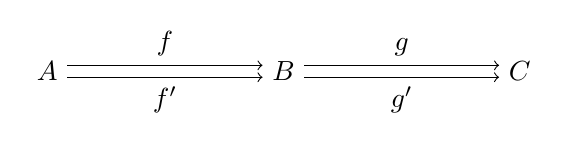
\begin{tikzpicture}
          \node (A)              {$A$};
          \node (B) [right of=A] {$B$};
          \node (C) [right of=B] {$C$};
          \draw[->,transform canvas={yshift=0.5ex}]  (A) to node {$f$} (B);
          \draw[->,transform canvas={yshift=-0.5ex}] (A) to node[anchor=north] {$f'$} (B);
          \draw[->,transform canvas={yshift=0.5ex}]  (B) to node {$g$} (C);
          \draw[->,transform canvas={yshift=-0.5ex}] (B) to node[anchor=north] {$g'$} (C);
        \end{tikzpicture}
      \end{figure}
    \end{theorem}
    \begin{proof}
      By definition of congruence, $f \sim f'$ implies $g \circ f \circ 1_A \sim g \circ f' \circ 1_A$ or simply $g \circ f \sim g \circ f'$.

      By definition of congruence, $g \sim g'$ implies $1_C \circ g \circ f \sim 1_A \circ g' \circ f$ or simply $g \circ f \sim g' \circ f$.

      By transitivity of congruence, $g \circ f \sim g' \circ f'$.
    \end{proof}

\end{enumerate}

\end{document}
